\chapter{Specifikacija programske potpore}
		
	\section{Funkcionalni zahtjevi}
			
	%		\textbf{\textit{dio 1. revizije}}\\
		    
		%	\par{Navesti \textbf{dionike} koji imaju \textbf{interes u ovom sustavu} ili  \textbf{su nositelji odgovornosti}. To su prije svega korisnici, ali i administratori sustava, naručitelji, razvojni tim.}\\
				
	%		\textit{Navesti \textbf{aktore} koji izravno \textbf{koriste} ili \textbf{komuniciraju sa sustavom}. Oni mogu imati inicijatorsku ulogu, tj. započinju određene procese u sustavu ili samo sudioničku ulogu, tj. obavljaju određeni posao. Za svakog aktora navesti funkcionalne zahtjeve koji se na njega odnose.}\\
			
			
			\noindent \textbf{Dionici:}
			
			\begin{packed_enum}
				
				\item Naručitelj projekta (zavod za javno zdravstvo, Crveni križ...)
				\item Razvojni tim
				\item Donori
				\item Djelatnici banke krvi
				\item Administratori sustava
				\item Svi korisnici interneta koji koriste javnu stranicu sustava radi pregleda trenutne razine krvi
				
			\end{packed_enum}
			
			\noindent \textbf{Aktori i njihovi funkcionalni zahtjevi:}
			
			
			\begin{packed_enum}
				\item  \underbar{Administrator (inicijator) može:}
				
				\begin{packed_enum}
					
					\item Administrirati korisničke račune:
					\begin{packed_enum}
						
						\item  Dodati račun djelatnika banke
				    	\item Deaktivirati bilo koji račun u sustavu
				    	\item Definirati optimalne granice razina krvi
				
					\end{packed_enum}
					
				\end{packed_enum}
			
				\item  \underbar{Djelatnik banke (inicijator) može:}
				
				\begin{packed_enum}
					
					\item Prikupiti podatke o donoru
					\begin{packed_enum}
						
						\item Prikupiti matične i kontakt podatke
						\item Prikupiti zdravstvene podatke (krvna grupa)
				
					\end{packed_enum}
					\item Stvoriti korisnički račun donora
					\item Nadopuniti podatke postojećeg računa donora (ukljućujući i zdravstvene podatke)
					\item Evidentirati pokušaj doniranja
					\begin{packed_enum}
						
						\item Zabilježiti trenutne zdravstvene podatke o donoru
						\item  Zabilježiti uspješnost pokušaja doniranja
				
					\end{packed_enum}
					\item Evidentirati trajno odbijanje donora (postojanje + razlog)
					\item Povećati zalihu krvi u sustavu uspješnim doniranjem
					\item Evidentirati slanje krvi u vanjsku instituciju (bolnicu)
					
				\end{packed_enum}
				
				\item  \underbar{Djelatnik banke (sudionik) može:}
				
				\begin{packed_enum}
					
					\item Primiti obavijest o prekoračenju bilo koje od optimalnih granica zaliha krvi
					\item Primiti aktivacijski link radi aktivacije računa
					
				\end{packed_enum}
				
				\item  \underbar{Donor (inicijator) može:}
				
				\begin{packed_enum}
					
					\item Krearati svoj korisnički račun prije prvog darivanja
					\item Nadopuniti podatke računa (osim zdravstvenih podataka - krvne grupe i trajnog odbijanja)
					\item Pregledati povijest darivanja krvi
					\item Preuzeti PDF potvrdu o postojećem doniranju krvi
					
				\end{packed_enum}
				
				
				\item  \underbar{Donor (sudionik) može:}
				
				\begin{packed_enum}
					
					\item Primiti aktivacijski link radi aktivacije računa
					\item Dobiti generirani donorID
					\item Primiti upozorenje o prekoračenju donje optimalne granice zaliha krvi (ako donor nije trajno odbijen)
					\item Pri spajanju u sustav dobiti informaciju o trenutnim zalihama krvi svoje krvne grupe (ako donor nije trajno odbijen)
					\item Primiti obavijest o isteku perioda zabrane darivanja u trajanju od 3 do 4 mjeseca od zadnjeg darivanja
					\item Primiti e-mail s PDF potvrdom o darivanju (nakon darivanja i nakon vlastitog iniciranja izdavanja potvrde)
					
				\end{packed_enum}
				
				\item  \underbar{Korisnik javnog weba (inicijator) može:}
				
				\begin{packed_enum}
					
					\item Krearati novi korisnički račun donora
					\item Pregledati trenutno stanje zaliha krvi svake krvne grupe
					
				\end{packed_enum}
				
				\item  \underbar{Baza podataka (inicijator) može:}
				
				\begin{packed_enum}
					
					\item Izdati obavijest o isteku nedopuštenog perioda darivanja u trajanju od tri do četiri mjeseca
					
				\end{packed_enum}
				
				\item  \underbar{Baza podataka (sudionik) može:}
				
				\begin{packed_enum}
					
					\item Pohranjivati:
					
					    \begin{itemize}
					        \item Postojeće račune u sustavu
					        \item Podatke o donorima
					        \item Podatke o djelatnicima banke
					        \item Količine doza krvi svake krvne grupe u sustavu
					        \item Pokušaje doniranja i sve podatke vezane uz njih
					        \item Potrošnju krvi u sustavu
					    \end{itemize}
					
				\end{packed_enum}
				
			\end{packed_enum}
			
			\eject 
			
			
				
			\subsection{Obrasci uporabe}
				
				%\textbf{\textit{dio 1. revizije}}
				
				\subsubsection{Opis obrazaca uporabe}
				%	\textit{Funkcionalne zahtjeve razraditi u obliku obrazaca uporabe. Svaki obrazac je potrebno razraditi prema donjem predlošku. Ukoliko u nekom koraku može doći do odstupanja, potrebno je to odstupanje opisati i po mogućnosti ponuditi rješenje kojim bi se tijek obrasca vratio na osnovni tijek.}\\
					
                \par {
                    *Baza podataka sudionik je u svim obrascima uporabe, stoga ju ne navodimo zasebno u svakom obrascu (ako je u nekom obrascu posebno navedena, to je kako bi se naglasilo da je u tom obrascu baza podataka glavni sudionik)
                } \\ \\
					\noindent \underbar{\textbf{UC1.1 - Stvori novi račun donora}} \label{UC1.1}
					\begin{packed_item}
	
						\item \textbf{Glavni sudionik: }djelatnik banke
						\item  \textbf{Cilj:} Stvaranje novog računa donora u sustavu pri doniranju krvi
						\item  \textbf{Sudionici:} donor
						\item  \textbf{Preduvjet:} Donor nema stvoren račun, djelatnik je prijavljen u sustav (\hyperref[UC3.1]{UC3.1})
						\item  \textbf{Opis osnovnog tijeka:}
						
						\item[] \begin{packed_enum}
							\item Djelatnik banke otvara obrazac za stvaranje pokušaja doniranja
							\item Djelatnik banke otvara obrazac za stvaranje računa donora
							\item Djelatnik banke unosi potrebne podatke o donoru koje saznaje ispitivanjem (matični i kontakt podatci, krvna grupa)
							\item Djelatnik banke pokreće stvaranje računa klikom na gumb \textit{Kreiraj račun}
							\item Sustav validira podatke
							\item Sustav stvara račun u bazi podataka, baza podataka generira donorID
							\item Djelatniku banke na ekran se ispisuje poruka o uspješno izrađenom računu
							\item Pokreće se \hyperref[UC2]{UC2} (\textit{Pošalji e-mail za aktivaciju} - novom donoru)
						\end{packed_enum}
						
						\item  \textbf{Opis mogućih odstupanja:}
						
						\item[] \begin{packed_item}
	
							\item[2.a] Donor nema / ne zna neki od obveznih podataka
							\begin{packed_enum}
								\item Proces se neuspješno završava
							\end{packed_enum}
							
							\item[2.b] Donor ne zna svoju krvnu grupu
                            \begin{packed_enum}
							    \item Djelatnik banke testom određuje krvnu grupa donora
							    \item Djelatnik banke upisuje krvnu grupu u račun donora
							    \item Proces kreiranja računa nastavlja se gdje je i stao na koraku 2 osnovnog tijeka
                            \end{packed_enum}
						
							\item[4.a] Dani podatci su sintaksno pogrešni
							\begin{packed_enum}
								\item Sustav na ekran ispisuje poruku o neispravnosti unesenih podataka
								\item Proces se nastavlja na koraku 2 osnovnog tijeka
							\end{packed_enum}
							
							\item[4.b] Unesen je podatak koji je već evidentiran kod nekog drugog donora, a radi se o podatku koji mora biti jedinstven
							\begin{packed_enum}
								\item Sustav na ekran ispisuje poruku o nejedinstvenosti unesenog podatka
								\item Proces se nastavlja na koraku 2 osnovnog tijeka
							\end{packed_enum}
							
						\end{packed_item}
						
					\end{packed_item}
					
					\noindent \underbar{\textbf{UC1.2 - Stvori novi račun sebi}}
					\begin{packed_item}
	
						\item \textbf{Glavni sudionik: }donor
						\item  \textbf{Cilj:} Osobno stvaranje novog računa donora u sustavu
						\item  \textbf{Sudionici:} 
						\item  \textbf{Preduvjet:} Donor nema stvoren račun, donor ima pristup internetu
						\item  \textbf{Opis osnovnog tijeka:}
						
						\item[] \begin{packed_enum}
                        	\item Donor otvara obrazac za registraciju
							\item Donor unosi potrebne podatke (matični i kontakt podatci, ne i krvna grupa)
							\item Donor pokreće stvaranje računa klikom na gumb \textit{Kreiraj račun}
							\item Sustav validira podatke 
							\item Sustav stvara račun u bazi podataka, baza podataka generira donorID
							\item Donoru se na ekran ispisuje poruka o uspješno izrađenom računu
							\item Pokreće se \hyperref[UC2]{UC2} (\textit{Pošalji e-mail za aktivaciju} - novom donoru)
						\end{packed_enum}
						
						\item  \textbf{Opis mogućih odstupanja:}
						
						\item[] \begin{packed_item}
	
                        	\item[2.a] Donor nema / ne zna neki od obveznih podataka
							\begin{packed_enum}
								\item Proces se neuspješno završava
							\end{packed_enum}
						
							\item[4.a] Dani podatci su sintaksno pogrešni
							\begin{packed_enum}
								\item Sustav na ekran ispisuje poruku o neispravnosti unesenih podataka
								\item Proces se nastavlja na koraku 2 osnovnog tijeka
							\end{packed_enum}
							
							\item[4.b] Unesen je podatak koji je već evidentiran kod nekog drugog donora, a radi se o podatku koji mora biti jedinstven
							\begin{packed_enum}
								\item Sustav na ekran ispisuje poruku o nejedinstvenosti unesenog podatka
								\item Proces se nastavlja na koraku 2 osnovnog tijeka
							\end{packed_enum}
							
						\end{packed_item}
						
					\end{packed_item}
					
					\noindent \underbar{\textbf{UC1.3 - Stvori novi račun djelatnika banke}}
					\begin{packed_item}
	
						\item \textbf{Glavni sudionik: }administrator
						\item  \textbf{Cilj:} Stvaranje novog računa djelatnika banke u sustavu
						\item  \textbf{Sudionici:} djelatnik banke
						\item  \textbf{Preduvjet:} Djelatnik banke nema stvoren račun, administrator ima sve potrebne podatke, administrator je prijavljen u sustav (\hyperref[UC3.1]{UC3.1})
						\item  \textbf{Opis osnovnog tijeka:}
						
						\item[] \begin{packed_enum}
                        	\item Administrator otvara obrazac za stvaranje računa djelatnika banke
							\item Administrator unosi potrebne podatke (matične i kontakt podatke djelatnika banke)
							\item Administrator pokreće stvaranje računa klikom na gumb \textit{Kreiraj račun}
							\item Sustav validira podatke 
							\item Sustav stvara račun u bazi podataka, baza podataka generira bankworkerID
							\item Administratoru se na ekran ispisuje poruka o uspješno izrađenom računu djelatnika
							\item Pokreće se \hyperref[UC2]{UC2} (\textit{Pošalji e-mail za aktivaciju} - novom djelatniku banke)
						\end{packed_enum}
						
						\item  \textbf{Opis mogućih odstupanja:}
						
						\item[] \begin{packed_item}
	
                        	\item[2.a] Administrator nema / ne zna neki od obveznih podataka
							\begin{packed_enum}
								\item Proces se neuspješno završava
							\end{packed_enum}
						
							\item[4.a] Dani podatci su sintaksno pogrešni
							\begin{packed_enum}
								\item Sustav na ekran ispisuje poruku o neispravnosti unesenih podataka
								\item Proces se nastavlja na koraku 2 osnovnog tijeka
							\end{packed_enum}
							
							
							\item[4.b] Unesen je podatak koji je već evidentiran kod nekog drugog djelatnika banke, a radi se o podatku koji mora biti jedinstven
							\begin{packed_enum}
								\item Sustav na ekran ispisuje poruku o nejedinstvenosti unesenog podatka
								\item Proces se nastavlja na koraku 2 osnovnog tijeka
							\end{packed_enum}
							
						\end{packed_item}
						
					\end{packed_item}
					
					%\noindent \underbar{\textbf{UC1.4 - Stvori novi račun administratora}}
					%\begin{packed_item}
	
					%	\item \textbf{Glavni sudionik: }administrator
					%	\item  \textbf{Cilj:} Stvaranje novog računa administratora u sustavu
					%	\item  \textbf{Sudionici:} 
					%	\item  \textbf{Preduvjet:} Postoji bar jedan administrator u sustavu, administrator je prijavljen u sustav (\hyperref[UC3.1]{UC3.1})
					%	\item  \textbf{Opis osnovnog tijeka:}
						
					%	\item[] \begin{packed_enum}
                    %    	\item Administrator otvara obrazac za stvaranje računa administratora
					%		\item Administrator unosi e-adresu novog administratora (koja se ne sprema trajno)
					%		\item Administrator pokreće stvaranje računa klikom na gumb \textit{Kreiraj račun}
					%		\item Sustav validira e-adresu 
					%		\item Sustav stvara račun u bazi podataka (generira lozinku), baza podataka generira userID
					%		\item Administratoru se na ekran ispisuje generirani userID
					%		\item Pokreće se \hyperref[UC2]{UC2} (Pošalji e-mail za aktivaciju - novom administratoru)
					%	\end{packed_enum}

					%	\item  \textbf{Opis mogućih odstupanja:}
						
					%	\item[] \begin{packed_item}
	
					%		\item[4] E-adresa je sintaksno pogrešna
					%		\begin{packed_enum}
					%			\item Sustav na ekran ispisuje poruku o neispravnosti e-adrese
					%			\item Proces se nastavlja na koraku 2 osnovnog tijeka
					%		\end{packed_enum}
							
					%	\end{packed_item}
						
					%\end{packed_item}
					
					\noindent \underbar{\textbf{UC2 - Pošalji e-mail za aktivaciju}}
					\begin{packed_item} \label{UC2}
	
						\item \textbf{Glavni sudionik: } korisnik sustava (donor, djelatnik banke ili administrator)
						\item  \textbf{Cilj:} Poslati e-mail s korisničkim podatcima i poveznicom za aktivaciju računa
						\item  \textbf{Sudionici:} 
						\item  \textbf{Preduvjet:} Novi korisnik pokrenuo je stvaranje računa; sustav ima generirane userID i inicijalnu lozinku
						\item  \textbf{Opis osnovnog tijeka:}
						
						\item[] \begin{packed_enum}
	                        \item Sustav generira poveznicu za aktivaciju računa
	                        \item Sustav generira e-poruku s navedenom poveznicom za aktivaciju te inicijalnim podatcima za prijavu
	                        \item Sustav na e-adresu definiranu pri kreiranju računa šalje e-poruku s generiranim podatcima
						\end{packed_enum}
						
						\item  \textbf{Opis mogućih odstupanja:}
						
					\end{packed_item}
					
					
					\noindent \underbar{\textbf{UC3 - Aktiviraj svoj račun}}
					\begin{packed_item}  \label{UC3}
	
						\item \textbf{Glavni sudionik: }novi korisnik sustava (donor, djelatnik banke ili administrator)
						\item  \textbf{Cilj:} Aktivirati korisnički račun radi buduće prijave u sustav
						\item  \textbf{Sudionici:} 
						\item  \textbf{Preduvjet:} Novi korisnik sustava ima generiran račun, korisnički podatci dostavljeni su na e-adresu, korisnik sustava ima pristup korisničkim podatcima
						\item  \textbf{Opis osnovnog tijeka:}
						
						\item[] \begin{packed_enum}
	
	                        \item Korisnik pristupa poveznici za aktivaciju računa
	                        \item Sustav u bazi podataka evidentira račun kao aktiviran

						\end{packed_enum}
						
						\item  \textbf{Opis mogućih odstupanja:}
						
					\end{packed_item}
					
					\noindent \underbar{\textbf{UC3.1 - Prijavi se u sustav}}
					\begin{packed_item}  \label{UC3.1}
	
						\item \textbf{Glavni sudionik: }korisnik sustava
						\item  \textbf{Cilj:} Prijaviti se u sustav i dobiti pristup značajkama dostupnima samo prijavljenim korisnicima
						\item  \textbf{Sudionici:} 
						\item  \textbf{Preduvjet:} Korisnik sustava ima generiran račun, korisnik sustava ima pristup korisničkim podatcima
						\item  \textbf{Opis osnovnog tijeka:}
						
						\item[] \begin{packed_enum}
	                        \item Korisnik na početnoj stranici pritišće gumb \textit{Prijavi se}
	                        \item Korisnik u polja za prijavu unosi svoj userID (donorID, bankworkerID) i lozinku
	                        \item Korisnik pritiskom na gumb \textit{Prijava} pokreće proces prijave u sustav
	                        \item Sustav provjerava ispravnost podataka i nakon potvrde vraća kolačić s identifikatorom sjednice
	                        \item Sustav preusmjerava korisnika na početnu stranicu profila
						\end{packed_enum}
						
						\item  \textbf{Opis mogućih odstupanja:}
						\item[] \begin{packed_enum}
						
	                        \item[4.a] Korisnik nema aktiviran račun
	                        \item[] \begin{packed_enum}
    	                        \item Sustav na ekran ispisuje poruku o nemogućnosti prijave zbog neaktiviranog računa
    	                        \item Proces se prekida
					    	\end{packed_enum}
					    	
	                        \item[4.b] Korisnik je unio neki od pogrešnih podataka za prijavu
	                        \item[] \begin{packed_enum}
    	                        \item Sustav na ekran ispisuje poruku o nemogućnosti prijave zbog neispravnih podataka za prijavu
    	                        \item Proces se nastavlja na koraku 2 osnovnog tijeka
					    	\end{packed_enum}
						\end{packed_enum}
						
					\end{packed_item}
					
						
					\noindent \underbar{\textbf{UC4 - Pregledaj svoje podatke}}
					\begin{packed_item}  \label{UC4}
	
						\item \textbf{Glavni sudionik: }donor
						\item  \textbf{Cilj:} Pregledati podatke računa trenutnog korisnika
						\item  \textbf{Sudionici:} djelatnik banke
						\item  \textbf{Preduvjet:} Trenutni korisnik ima račun i prijavljen je u sustav (\hyperref[UC3.1]{UC3.1})
						\item  \textbf{Opis osnovnog tijeka:}
						
						\item[] \begin{packed_enum}
	
	                        \item Korisnik na podstranici \textit{Profil} pritišće gumb \textit{Uredi podatke}
	                        \item Sustav učitava stranicu s postojećim podatcima i gumbom za uređivanje podataka

						\end{packed_enum}
						
						\item  \textbf{Opis mogućih odstupanja:}

						
					\end{packed_item}
					
					
					\noindent \underbar{\textbf{UC4.1 - Pronađi i pregledaj podatke donora}}
					\begin{packed_item}  \label{UC4.1}
	
						\item \textbf{Glavni sudionik: }djelatnik banke
						\item  \textbf{Cilj:} Pronaći donora u sustavu i pregledati njegove podatke
						\item  \textbf{Sudionici:} administrator
						\item  \textbf{Preduvjet:} Donor ima generiran račun, trenutni korisnik je prijavljen u sustav (\hyperref[UC3.1]{UC3.1}) i ima dovoljno podataka o donoru kako bi ga pronašao u sustavu
						\item  \textbf{Opis osnovnog tijeka:}
						\\ *Korisnikom se smatra djelatnik banke ili administrator
						\item[] \begin{packed_enum}
	                    
	                        \item Korisnik pristupa obrascu za traženje donora klikom na gumb \textit{Pronađi donora} na stranici za stvaranje pokušaja doniranja ili na stranici za deaktivaciju računa
	                        \item Korisnik u obrazac unosi neki od podataka donora (donorID, OIB, ime, prezime) ili više njih u kombinaciji, odvojene razmakom
	                        \item Sustav iz baze podataka dobavlja podatke o traženim donorima
	                        \item Sustav u tabličnom prikazu ispisuje sve donore kojima se osobni podatci podudaraju s traženima
	                        \item Korisnik odabire željenog donora klikom na željeni redak
	                        \item Sustav preusmjerava korisnika na prethodnu stranicu s koje je došao, pritom noseći i podatak o odabranom donoru

						\end{packed_enum}
						
						\item  \textbf{Opis mogućih odstupanja:}
						\item[] \begin{packed_item}
	
							\item[3.1] Sustav od baze podataka ne dobiva podatke jer ne postoji donor s navedenim podatcima
							\item[] \begin{packed_enum}
								\item Sustav na ekran ispisuje da nema pronađenih rezultata
								\item Izvođenje se nastavlja na koraku 2 osnovnog tijeka
							\end{packed_enum}
							\item[3.2] Traženi račun je trajno deaktiviran
							\item[] \begin{packed_enum}
								\item Sustav iz baze podataka dobavlja podatke samo o nedeaktiviranim korisnicima
								\item Baza podataka ne pronalazi zapis traženog donora
								\item Sustav na ekran ispisuje da nema pronađenih rezultata
								\item Izvođenje se nastavlja na koraku 2 osnovnog tijeka
							\end{packed_enum}
							
						\end{packed_item}
						
					\end{packed_item}
					
					
					\noindent \underbar{\textbf{UC4.2 - Pronađi i pregledaj podatke djelatnika banke}}
					\begin{packed_item}  \label{UC4.2}
	
						\item \textbf{Glavni sudionik: }administrator
						\item  \textbf{Cilj:} Pronaći djelatnika banke u sustavu i pregledati njegove podatke
						\item  \textbf{Sudionici:} 
						\item  \textbf{Preduvjet:} Djelatnik ima generiran račun, administrator je prijavljen u sustav (\hyperref[UC3.1]{UC3.1}), administrator ima dovoljno podataka o djelatniku banke kako bi ga pronašao u sustavu
						\item  \textbf{Opis osnovnog tijeka:}
						
						\item[] \begin{packed_enum}
	                        \item Administrator pristupa obrascu za traženje djelatnika banke klikom na gumb \textit{Pronađi djelatnika} sa stranice za deaktivaciju računa
	                        \item Administrator u obrazac unosi neki od podataka donora (donorID, OIB, ime, prezime) ili više njih u kombinaciji, odvojene razmakom
	                        \item Sustav iz baze podataka dobavlja podatke o traženim djelatnicima banke
	                        \item Sustav u tabličnom prikazu ispisuje sve djelatnike banke kojima se osobni podatci podudaraju s traženima
	                        \item Administrator odabire željenog djelatnika banke klikom na željeni redak
	                        \item Sustav preusmjerava administratora na prethodnu stranicu s koje je došao, pritom noseći i podatak o odabranom djelatniku banke
						\end{packed_enum}
						
						\item  \textbf{Opis mogućih odstupanja:}
						\item[] \begin{packed_item}
	
							\item[3.1] Sustav od baze podataka ne dobiva podatke jer ne postoji djelatnik banke s navedenim podatcima
							\item[] \begin{packed_enum}
								\item Sustav na ekran ispisuje poruku o neuspješnom dohvaćanju djelatnika banke
								\item Izvođenje se nastavlja na koraku 2 osnovnog tijeka
							\end{packed_enum}
							\item[3.2] Traženi račun je trajno deaktiviran
							\item[] \begin{packed_enum}
								\item Sustav iz baze podataka dobavlja podatke samo o nedeaktiviranim korisnicima
								\item Baza podataka ne pronalazi zapis traženog djelatnika banke
								\item Sustav na ekran ispisuje da nema pronađenih rezultata
								\item Izvođenje se nastavlja na koraku 2 osnovnog tijeka
							\end{packed_enum}
							
						\end{packed_item}
						
					\end{packed_item}
					
					
					\noindent \underbar{\textbf{UC5 - Uredi matične i kontakt podatke donora}}
					\begin{packed_item} \label{UC5}
	
						\item \textbf{Glavni sudionik: }donor
						\item  \textbf{Cilj:} Uređivanje svojih postojećih matičnih i kontakt podataka
						\item  \textbf{Sudionici:} 
						\item  \textbf{Preduvjet: }Donor ima stvoren račun i nalazi se na stranici za uređivanje osobnih podataka (vidi \hyperref[UC4]{UC4 (\textit{Pregledaj svoje podatke})}
						\item  \textbf{Opis osnovnog tijeka:}
						
						\item[] \begin{packed_enum}
	                        \item Donor izmjenjuje potrebne matične ili kontakt podatake (ali ne i zdravstvene podatke)
	                        \item Donor pritišće gumb \textit{Pohrani promjene}
	                        \item Sustav validira ispravnost podataka
	                        \item Sustav ažurira postojeći zapis u bazi podataka
	                        
						\end{packed_enum}
						
						\item  \textbf{Opis mogućih odstupanja:}
						
						\item[] \begin{packed_item}
	
							\item[4.a] Donor želi promijeniti OIB na vrijednost koja više ne bi bila jedinstvena
							\begin{packed_enum}
								\item Sustav ispisuje poruku o nejedinstvenosti podatka te odbija spremiti promjene
								\item Proces se nastavlja na koraku 2 osnovnog tijeka
							\end{packed_enum}
							
							\item[4.b] Dani podatci su sintaksno pogrešni
							\begin{packed_enum}
								\item Sustav na ekran ispisuje poruku o neispravnosti unesenih podataka
								\item Proces se nastavlja na koraku 2 osnovnog tijeka
							\end{packed_enum}
							
						\end{packed_item}
						
					\end{packed_item}
					
					\noindent \underbar{\textbf{UC5.1 - Uredi zdravstvene, matične i kontakt podatke donora}}
					\begin{packed_item} \label{UC5.1}
	
						\item \textbf{Glavni sudionik: }djelatnik banke
						\item  \textbf{Cilj:} Uređivanje postojećih podataka o računu donora
						\item  \textbf{Sudionici:} donor
						\item  \textbf{Preduvjet:} Donor ima stvoren račun, djelatnik banke ga je pronašao koristeći \hyperref[UC4.1]{UC4.1 (\textit{Pronađi i pregledaj podatke donora})} 
						\item  \textbf{Opis osnovnog tijeka:}
						
						\item[] \begin{packed_enum}
	                        \item Djelatnik banke sa stranice za stvaranje pokušaja donacije pristupa obrascu za izmjenu podataka donora klikom na gumb \textit{Uredi podatke}
	                        \item Djelatnik izmjenjuje bilo koji potrebni podatak o donoru  (uključujući i zdravstvene podatke)
	                        \item Djelatnik pritišće gumb \textit{Pohrani promjene}
	                        \item Sustav validira ispravnost podataka
	                        \item Sustav ažurira postojeći zapis u bazi podataka
	                      %  \item U slučaju neaktualnih podataka, djelatnik banke ažurira podatke
	                      % \item U slučaju da je donor sam stvorio račun, provjerava se krvna grupa donora i djelatnik banke ju unosi u sustav
	                      %  \item Ukoliko se pri evidenciji zdravstvenih podataka u pokušaju doniranja pokaže okolnost za trajno odbijanje donora, pokreće se \hyperref[UC4.3]{UC4.3} (\textit{Evidentiraj trajno odbijanje donora})
						\end{packed_enum}
						
						\item  \textbf{Opis mogućih odstupanja:}
						
						\item[] \begin{packed_item}
	
							\item[4.a] Djelatnik banke želi promijeniti OIB donora na vrijednost koja više ne bi bila jedinstvena
							\begin{packed_enum}
								\item Sustav ispisuje poruku o nejedinstvenosti podatka te odbija spremiti promjene
								\item Proces se nastavlja na koraku 2 osnovnog tijeka
							\end{packed_enum}
							
							\item[4.b] Dani podatci su sintaksno pogrešni
							\begin{packed_enum}
								\item Sustav na ekran ispisuje poruku o neispravnosti unesenih podataka
								\item Proces se nastavlja na koraku 2 osnovnog tijeka
							\end{packed_enum}
							
						\end{packed_item}
						
					\end{packed_item}
					
				
					\noindent \underbar{\textbf{UC5.2 - Uredi podatke djelatnika banke}}
					\begin{packed_item}
	
						\item \textbf{Glavni sudionik: }djelatnik banke
						\item  \textbf{Cilj:} Uređivanje već postojećih podataka 
						\item  \textbf{Sudionici:} 
						\item  \textbf{Preduvjet: }Djelatnik banke ima stvoren račun i nalazi se na stranici za uređivanje osobnih podataka (vidi \hyperref[UC4]{UC4 (\textit{Pregledaj svoje podatke})}
						\item  \textbf{Opis osnovnog tijeka:}
						
						\item[] \begin{packed_enum}
	                        \item Djelatnik banke izmjenjuje potrebni podatak 
	                        \item Djelatnik banke pritišće gumb \textit{Pohrani promjene}
	                        \item Sustav validira ispravnost podataka
	                        \item Sustav ažurira postojeći zapis u bazi podataka
	                        
						\end{packed_enum}
						
						\item  \textbf{Opis mogućih odstupanja:}
						
						\item[] \begin{packed_item}
	
							\item[4.a] Djelatnik banke želi promijeniti OIB na vrijednost koja više ne bi bila jedinstvena
							\begin{packed_enum}
								\item Sustav ispisuje poruku o nejedinstvenosti podatka te odbija spremiti promjene
								\item Proces se nastavlja na koraku 2 osnovnog tijeka
							\end{packed_enum}
							
							\item[4.b] Dani podatci su sintaksno pogrešni
							\begin{packed_enum}
								\item Sustav na ekran ispisuje poruku o neispravnosti unesenih podataka
								\item Proces se nastavlja na koraku 2 osnovnog tijeka
							\end{packed_enum}
							
						\end{packed_item}
						
					\end{packed_item}
					
					
					\noindent \underbar{\textbf{UC5.3 - Deaktiviraj račun}}
					\begin{packed_item} \label{5.3}
	
						\item \textbf{Glavni sudionik: }administrator
						\item  \textbf{Cilj:} Deaktivacija postojećeg računa 
						\item  \textbf{Sudionici:} 
						\item  \textbf{Preduvjet:} Korisnički račun koji se treba deaktivirati postoji
						\item  \textbf{Opis osnovnog tijeka:}
						
						\item[] \begin{packed_enum}
	
	                        \item Administrator pristupa stranici za deaktivaciju računa pritiskom na gumb \textit{Upravljaj računima}
	                        \item Administrator koristi tražilicu kako bi pronašao traženi račun pritiskom na gumb \textit{Pronađi donora} ili \textit{Pronađi djelatnika} (vidi \hyperref[UC4.1]{UC4.1 (\textit{Pronađi i pregledaj podatke donora})} ili \hyperref[UC4.2]{UC4.2 (\textit{Pronađi i pregledaj podatke djelatnika banke})})
							\item Administrator nakon pronalaska računa i povratka na stranicu za deaktivaciju pritišće gumb \textit{Deaktiviraj račun}
	                        \item Sustav u bazi podataka evidentira da je račun deaktiviran (ali račun se ne briše)

						\end{packed_enum}
						
						\item  \textbf{Opis mogućih odstupanja:}
						
					\end{packed_item}
					
					
					\noindent \underbar{\textbf{UC6 - Stvori pokušaj doniranja}}
					\begin{packed_item} \label{UC6}
	
						\item \textbf{Glavni sudionik: }djelatnik banke
						\item  \textbf{Cilj:} Stvaranje pokušaja doniranja, evidentiranje trenutnih zdravstvenih podataka
						\item  \textbf{Sudionici:} donor
						\item  \textbf{Preduvjet:} Donor je došao na doniranje i ima izrađen korisnički račun 
						\item  \textbf{Opis osnovnog tijeka:}
						
						\item[] \begin{packed_enum}
	
							\item Djelatnik banke otvara obrazac za unos novog pokušaja darivanja
							\item Djelatnik banke pronalazi donora u sustavu koristeći tražilicu pritiskom na gumb \textit{Pronađi donora} - vidi \hyperref[UC4.1]{UC4.1 (\textit{Pronađi i pregledaj podatke donora})}
							\item Djelatnik banke u sustavu ispunjava zdravstveni upitnik prema odgovorima koje mu daje donor
	                        \item Djelatnik pritiskom na gumb \textit{Spremi pokušaj doniranja} pokreće proces spremanja
	                        \item Donor odlazi darivati krv, a pokušaj doniranja evidentira se kao uspješan
	                        \item Sustav u bazi podataka stvara novi pokušaj doniranja s prethodno navedenim podatcima
	                        \item Sustav u bazi podataka evidentira povećanje zalihe krvi krvne grupe donora iz ovog pokušaja za jednu dozu
	                        \item Sustav generira PDF potvrdu o darivanju krvi
	                        \item Djelatniku se na ekran ispisuje poruka o uspješnom darivanju krvi
	                        \item Sustav šalje potvrdu na mail (vidi \hyperref[UC12]{UC12} za sličnu funkcionalnost gdje se potvrda preuzima na računalo)

						\end{packed_enum}
						
						\item  \textbf{Opis mogućih odstupanja:}
						
						\item[] \begin{packed_item}
	
							\item[4.a] Neki od zdravstvenih podataka implicira privremeno odbijanje donora
							\begin{packed_enum}
								\item Djelatnik pokušaj doniranja evidentira kao neuspješan
								\item Obavlja se korak 6 osnovnog tijeka (spremanje pokušaja doniranja)
								\item Djelatniku se na ekran ispisuje poruka o neuspješnom darivanju krvi
								\item Proces završava
							\end{packed_enum}
							
							\item[4.b] Neki od zdravstvenih podataka implicira trajno odbijanje donora
							\begin{packed_enum}
								\item Sustav pokušaj doniranja evidentira kao neuspješan
								\item Sustav evidentira trajno odbijanje u računu donora s razlogom odbijanja poslanom u obrascu
								\item Obavlja se korak 6 osnovnog tijeka (spremanje pokušaja doniranja)
								\item Djelatniku se na ekran ispisuje poruka o neuspješnom darivanju krvi
								\item Proces završava
							\end{packed_enum}
							
							\item[7] S novom dozom krvi prekoračuje se gornja optimalna granica zaliha doza krvi
							\begin{packed_enum}
							    \item Pokreće se \hyperref[UC14]{UC14 (\textit{Izdaj upozorenje o prekoračenju optimalne granice})}
								\item Proces se nastavlja gdje je i stao na koraku 7 osnovnog tijeka
							\end{packed_enum}
							
						\end{packed_item}
						
					\end{packed_item}
					
					
					\noindent \underbar{\textbf{UC7 - Pregledaj zalihe svih krvnih grupa}}
					\begin{packed_item}
	
						\item \textbf{Glavni sudionik: }korisnik interneta
						\item  \textbf{Cilj:} Na javnom webu pregledati stanja svih krvnih grupa i dobiti informaciju o stanju zaliha svake grupe u odnosu na optimalne granice
						\item  \textbf{Sudionici:}
						\item  \textbf{Preduvjet:} 
						\item  \textbf{Opis osnovnog tijeka:}
						
						\item[] \begin{packed_enum}
	
	                        \item Korisnik interneta pristupa početnoj stranici aplikacije
	                        \item Sustav dohvaća trenutna stanja zaliha krvi i optimalne granice za svaku krvnu grupu iz baze podataka
	                        \item Sustav vizualno prikazuje stanja zaliha svih krvnih grupa i njihovih optimalnih granica tako da je gornja optimalna granica na 90\% visine, donja optimalna granica i trenutna razina krvi proporcionalno tome (donja optimalna granica na visini od donjaGranica/gornjaGranica*90\%, a trenutna razina krvi na visini od razina/gornjaGranica*90\%)
	                        \item Sustav provjerava nalaze li se sva stanja zaliha između optimalnih granica

						\end{packed_enum}
						
						\item  \textbf{Opis mogućih odstupanja:}
						
						\item[] \begin{packed_item}
	
							\item[4] Neko stanje zaliha nalazi se ispod donje optimalne granice za tu krvnu grupu 
							\begin{packed_enum}
								\item Sustav na stranici ispisuje i poruku o nedostatku krvnih grupa čije je stanje ispod donje optimalne granice
								\item Proces završava
							\end{packed_enum}
							
						\end{packed_item}
						
					\end{packed_item}
					
					
					%\noindent \underbar{\textbf{UC8 - Promijeni lozinku}}
					%\begin{packed_item}
	
						%\item \textbf{Glavni sudionik: }prijavljeni korisnik
						%\item  \textbf{Cilj:} Promijeniti lozinku svog računa
						%\item  \textbf{Sudionici:} 
						%\item  \textbf{Preduvjet:} Korisnik ima podatke za prijavu, prijavljen je u sustav (\hyperref[UC3.1]{UC3.1}) i ima potrebu za promjenom lozinke
						%\item  \textbf{Opis osnovnog tijeka:}
						
						%item[] \begin{packed_enum}
	                        %\item Korisnik s profila otvara obrazac za promjenu lozinke pritiskom na gumb \textit{Promijeni lozinku}
	                        %\item Korisnik unosi staru i novu lozinku te pokreće validaciju i promjenu lozinke pritiskom na gumb \textit{Promijeni lozinku}
	                        %\item Sustav validira lozinku
	                        %\item Sustav u bazi podataka evidentira promjenu lozinke
	                        %\item Sustav korisniku na ekran ispisuje poruku o uspješno promijenjenoj lozinki
						%\end{packed_enum}
						
						%\item  \textbf{Opis mogućih odstupanja:}
						
						%\item[] \begin{packed_item}
	
							%\item[3] Lozinka je nesigurna (definirano u ostalim zahtjevima)
							%\begin{packed_enum}
								%\item Sustav na ekran ispisuje prikladnu poruku koja navodi korisnika na pravila za sastavljanje sigurne lozinke
								%\item Proces se nastavlja na koraku 2 osnovnog tijeka
							%\end{packed_enum}
							
						%\end{packed_item}
						
					%\end{packed_item}
					
					
					\noindent \underbar{\textbf{UC9 - Definiraj optimalne granice zaliha krvi}}
					\begin{packed_item} \label{UC9}
	
						\item \textbf{Glavni sudionik: }administrator
						\item  \textbf{Cilj:} Postaviti gornje i donje optimalne granice za svaku krvnu grupu
						\item  \textbf{Sudionici:} 
						\item  \textbf{Preduvjet:} Administrator ima korisnički račun i prijavljen je u sustav (\hyperref[UC3.1]{UC3.1})
						\item  \textbf{Opis osnovnog tijeka:}
						
						\item[] \begin{packed_enum}
							\item Administrator pristupa obrascu za postavljanje optimalnih granica pritiskom na gumb \textit{Uredi granice}
	                        \item Administrator za svaku krvnu grupu podešava gornje i donje optimalne granice zaliha krvi
	                        \item Administrator pokreće proces spremanja pritiskom na gumb \textit{Spremi granice}
	                        \item Sustav sprema promjene u bazu podataka
						\end{packed_enum}
						
						\item  \textbf{Opis mogućih odstupanja:}
						
						\item[] \begin{packed_item}
	
							\item[3] Administrator podešava novu donju optimalnu granicu iznad trenutne zalihe krvi, ili gornju optimalnu granicu ispod trenutne zalihe krvi za bilo koju krvnu grupu
							\item[] \begin{packed_enum}
                                \item Pokreće se \hyperref[UC14]{UC14 (\textit{Izdaj upozorenje o prekoračenju optimalne granice})}
                                \item Proces se nastavlja gdje je i stao na koraku 3 osnovnog tijeka
							\end{packed_enum}

						\end{packed_item}
						
					\end{packed_item}
					
					
					\noindent \underbar{\textbf{UC10 - Ispiši poruku o stanju zalihe krvne grupe donora}}
					\begin{packed_item}
	
						\item \textbf{Glavni sudionik: }donor
						\item  \textbf{Cilj:} Informirati donora o okvirnom stanju zaliha njegove krvne grupe
						\item  \textbf{Sudionici:} 
						\item  \textbf{Preduvjet:} Donor je prijavljen u sustav (\hyperref[UC3.1]{UC3.1}) i nedostaje njegove krvne grupe
						\item  \textbf{Opis osnovnog tijeka:}
						
						\item[] \begin{packed_enum}
	
							\item Donor dolazi na početnu stranicu prijavljenog korisnika (profil)
	                        \item Sustav na ekranu prikazuje poruku o nedostatku zalihe te krvne grupe

						\end{packed_enum}
						
						\item  \textbf{Opis mogućih odstupanja:}
						
						\item[] \begin{packed_item}
	
							\item[2] Stanje zaliha krvi je iznad donje optimalne granice
							\item[] \begin{packed_enum}
								\item Poruka se ne ispisuje
								\item Proces završava
							\end{packed_enum}
							
							\item[2] Stanje zaliha krvi je ispod donje optimalne granice
							\item[] \begin{packed_enum}
								\item Sustav ispisuje dodatno istaknutu poticajnu poruku za darivanje krvi
								\item Proces završava
							\end{packed_enum}

						\end{packed_item}
						
					\end{packed_item}
					
					
					\noindent \underbar{\textbf{UC11 - Pregledaj povijest pokušaja doniranja}}
					\begin{packed_item} \label{UC11}
	
						\item \textbf{Glavni sudionik: }donor
						\item  \textbf{Cilj:} Dati donoru uvid u sve svoje prijašnje pokušaje doniranja i njihov ishod, te ponuditi mogućnsot preuzimanja potvrde
						\item  \textbf{Sudionici:} djelatnik banke
						\item  \textbf{Preduvjet:} Donor je prijavljen u sustav (\hyperref[UC3.1]{UC3.1}) / djelatnik banke je pronašao donora u sustavu pri darivanju
						\item  \textbf{Opis osnovnog tijeka:}
						
						*Korisnikom se smatra donor ili djelatnik banke opisani u preduvjetima
						\item[] \begin{packed_enum}
							\item Korisnik otvara stranicu s povijesti pokušaja doniranja pritiskom na gumb \textit{Moje donacije / Prošle donacije}
	                        \item Sustav za svaki pokušaj doniranja navodi osnovne podatke definirane u ostalim zahtjevima
	                        \item Sustav za svaki uspješni pokušaj stvara i gumb \textit{Preuzmi}
						\end{packed_enum}
						
						\item  \textbf{Opis mogućih odstupanja:}
						
						\item[] \begin{packed_item}
	
							\item[2] Korisnik nema nijedan prethodan pokušaj doniranja
							\item[] \begin{packed_enum}
								\item Sustav ispisuje informativnu poruku o nepostojanju prijašnjih darivanja
								\item Proces završava
							\end{packed_enum}
							
							\item[3] Korisnik pritišće gumb \textit{Preuzmi} za neki pokušaj doniranja
							\item[] \begin{packed_enum}
							    \item Pokreće se (\hyperref[UC12]{UC12 - \textit{Preuzmi PDF potvrdu}}) od koraka 2 osnovnog tijeka
							\end{packed_enum}

						\end{packed_item}
						
					\end{packed_item}
					
					\noindent \underbar{\textbf{UC12 - Preuzmi PDF potvrdu}}
					\begin{packed_item} \label{UC12}
	
						\item \textbf{Glavni sudionik: }donor
						\item  \textbf{Cilj:} Preuzimanje PDF potvrde o pokušaju doniranja iz povijesti doniranja u sustavu
						\item  \textbf{Sudionici:} djelatnik
						\item  \textbf{Preduvjet:} Donor se nalazi na stranici s prethodnim pokušajima doniranja i ima obavljeno barem jedno uspješno doniranje / djelatnik banke pronašao je donora u sustavu i pristupio je stranici s njegovim prijašnjim donacijama (vidi \hyperref[UC11]{UC11})
						\item  \textbf{Opis osnovnog tijeka:}
						
						*Korisnikom se smatra donor ili djelatnik banke opisani u preduvjetima
						\item[] \begin{packed_enum}
	                        \item Korisnik pritišće gumb \textit{Preuzmi PDF potvrdu} 
	                        \item Sustav generira PDF potvrdu o doniranju
	                        \item Sustav pokreće preuzimanje PDF potvrde na računalo korisnika
						\end{packed_enum}
						
						\item  \textbf{Opis mogućih odstupanja:}
						
					\end{packed_item}
					
					
					\noindent \underbar{\textbf{UC13 - Evidentiraj slanje krvi u bolnicu}}
					\begin{packed_item} \label{UC13}
	
						\item \textbf{Glavni sudionik: }djelatnik banke
						\item  \textbf{Cilj:} Evidentirati smanjenje zalihe krvi radi slanja u bolnicu
						\item  \textbf{Sudionici:} 
						\item  \textbf{Preduvjet:} Djelatnik banke prijavljen je u sustav (\hyperref[UC3.1]{UC3.1})
						\item  \textbf{Opis osnovnog tijeka:}
						
						\item[] \begin{packed_enum}
	                        \item Djelatnik banke u sustavu otvara obrazac za slanje krvi u bolnicu pritiskom na gumb \textit{Slanje krvi}
                            \item Djelatnik banke popunjava broj doza koji se šalje od svake krvne grupe
                            \item Djelatnik banke inicira smanjenje zalihe krvi pritiskom na gumb \textit{Pošalji}
                        	\item Sustav u bazi podataka smanjuje zalihe krvi za odgovarajuće iznose
						\end{packed_enum}
						
						\item  \textbf{Opis mogućih odstupanja:}
						
						\item[] \begin{packed_item}
						
							\item[3] Djelatnik banke popunio je da se za neku krvnu grupu šalje više doza krvi nego što je postoji u sustavu
							\item[] \begin{packed_enum}
								\item Sustav djelatniku banke ispisuje poruku upozorenja o nemogućnosti slanja tolikog broja doza krvi 
								\item Proces se nastavlja na koraku 2 osnovnog tijeka
							\end{packed_enum}
							
							\item[4] Novo stanje krvi za bilo koju krvnu grupu nalazi se ispod, a prije je bilo iznad donje optimalne granice 
                            \item[] \begin{packed_enum} 
                                \item Pokreće se \hyperref[UC14]{UC14 (\textit{Izdaj upozorenje o prekoračenju optimalne granice})}
							\end{packed_enum}

						\end{packed_item}
						
					\end{packed_item}
					
					
					\noindent \underbar{\textbf{UC14 - Izdaj upozorenje o prekoračenju optimalne granice}}
					\begin{packed_item} \label{UC14}
	
						\item \textbf{Glavni sudionik: }djelatnik banke
						\item  \textbf{Cilj:} Upozoriti djelatnike banke u slučaju prekoračenja optimalnih granica zaliha krvi te upozoriti donore u slučaju prekoračenja donje optimalne granice
						\item  \textbf{Sudionici:} donor
						\item  \textbf{Preduvjet:} U sustavu postoje definirane optimalne granice zaliha krvi; dogodio se bar jedan od tri okidača u alternativnim slijedovima sljedećih obrazaca uporabe:
						\begin{packed_enum}
						    \item Evidentiranje slanja krvi u bolnicu (vidi \hyperref[UC13]{UC13})
						     \item Redefiniranje optimalnih granica (vidi \hyperref[UC9]{UC9})
						     \item Dodavanje nove doze krvi u sustav (vidi \hyperref[UC6]{UC6})
						\end{packed_enum}
						U osnovnom slijedu, pretpostavlja se da je zaliha krvi pala ispod donje optimalne granice:
						\item  \textbf{Opis osnovnog tijeka:}
						\item[] \begin{packed_enum}

	                        \item Sustav dohvaća e-adrese svih djelatnika banke iz baze podataka i izdaje im e-mail upozorenje o nedovoljnom stanju zaliha te krvne grupe 
	                        \item Sustav dohvaća e-adresu svih donora te krvne grupe koji nisu trajno odbijeni iz baze podataka i izdaje e-mail upozorenje o nedovoljnom stanju zaliha te krvne grupe s poticajem na doniranje 
	                       
    						
						\end{packed_enum}
						
						\item  \textbf{Opis mogućih odstupanja:}
						
						\item[] \begin{packed_item}
						
							\item[] Zaliha krvi nije pala ispod donje optimalne granice nego je narasla iznad gornje optimalne granice
							\item[] \begin{packed_enum} 
    	                        \item Sustav dohvaća e-adrese svih djelatnika banke iz baze podataka i izdaje im e-mail upozorenje o prevelikom stanju zaliha te krvne grupe 
    	                        \item Proces završava
							\end{packed_enum}

						\end{packed_item}
						
					\end{packed_item}
					
					
					\noindent \underbar{\textbf{UC15 - Izdaj obavijest o isteku perioda nemogućnosti doniranja}}
					\begin{packed_item}
	
						\item \textbf{Glavni sudionik: }baza podataka
						\item  \textbf{Cilj:} Obavijestiti donora o ponovnoj mogućnosti doniranja krvi
						\item  \textbf{Sudionici:} donor
						\item  \textbf{Preduvjet:} Donor je već darivao krv, započinje dan na datum na koji donoru istječe period nemogućnosti doniranja
						\item  \textbf{Opis osnovnog tijeka:}
						
						\item[] \begin{packed_enum}
							\item Sustav pokreće proces u kojemu računa periode od posljednjeg darivanja do današnjeg dana za svakog donora
	                        \item Sustav generira i šalje e-poruke za svakog donora kojemu je na taj dan istekao period nemogućnosti darivanja
						\end{packed_enum}
						
						\item  \textbf{Opis mogućih odstupanja:}
						
					\end{packed_item}
					
				\subsubsection{Dijagrami obrazaca uporabe}
					
				%	\textit{Prikazati odnos aktora i obrazaca uporabe odgovarajućim UML dijagramom. Nije nužno nacrtati sve na jednom dijagramu. Modelirati po razinama apstrakcije i skupovima srodnih funkcionalnosti.}
				
				\begin{figure}[H]
    			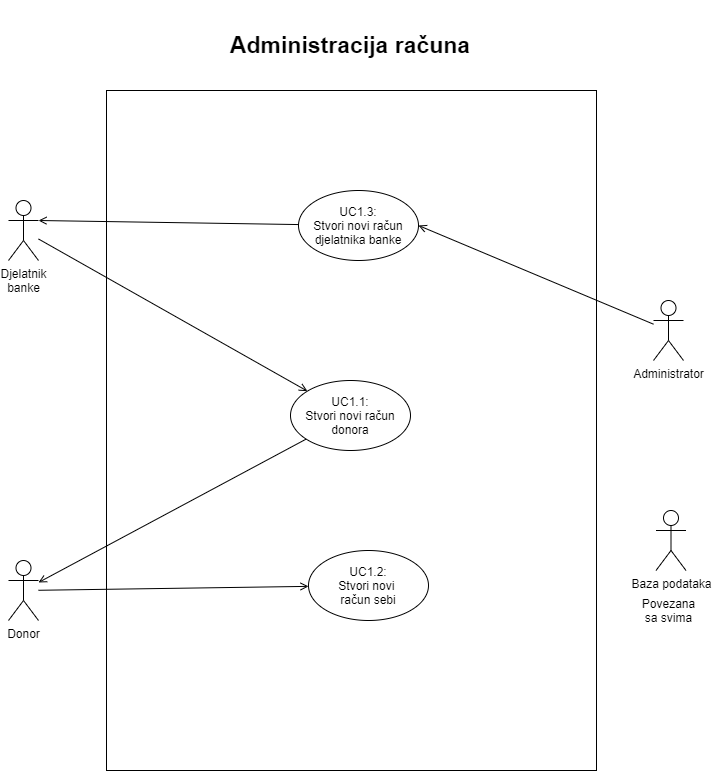
\includegraphics[scale=0.6]{slike/UC1.png} %veličina slike u odnosu na originalnu datoteku i pozicija slike
    			\centering
    			\caption{Dijagram obrazaca uporabe 1 - Administracija računa}
    			\label{fig:promjene}
    	    	\end{figure}
    	    	
				\begin{figure}[H]
    			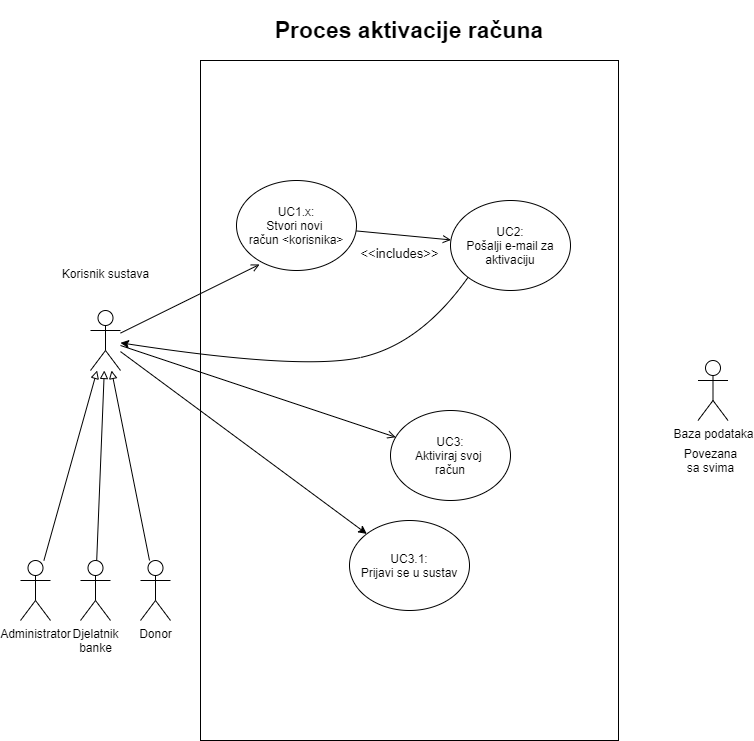
\includegraphics[scale=0.6]{slike/UC2.png} %veličina slike u odnosu na originalnu datoteku i pozicija slike
    			\centering
    			\caption{Dijagram obrazaca uporabe 2 - Proces aktivacije računa}
    			\label{fig:promjene}
    	    	\end{figure}
    	    	
				\begin{figure}[H]
    			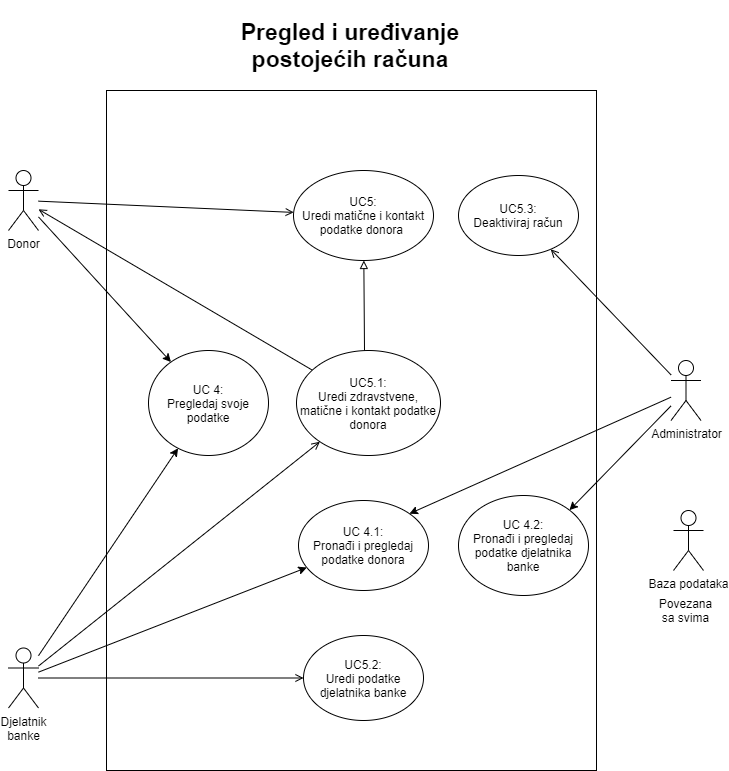
\includegraphics[scale=0.6]{slike/UC3.png} %veličina slike u odnosu na originalnu datoteku i pozicija slike
    			\centering
    			\caption{Dijagram obrazaca uporabe 3 - Uređivanje postojećih računa}
    			\label{fig:promjene}
    	    	\end{figure}
    	    	
				\begin{figure}[H]
    			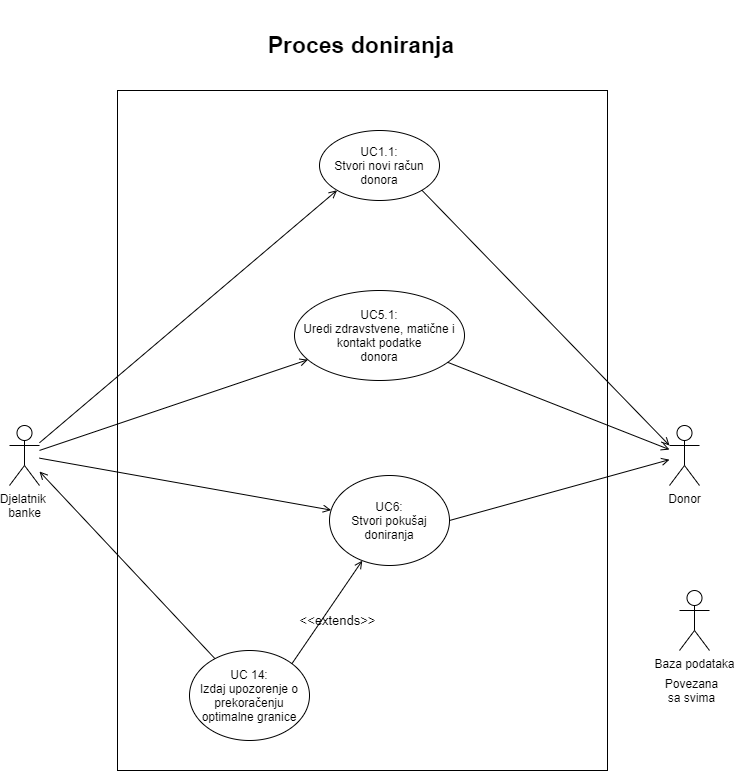
\includegraphics[scale=0.6]{slike/UC4.png} %veličina slike u odnosu na originalnu datoteku i pozicija slike
    			\centering
    			\caption{Dijagram obrazaca uporabe 4 - Proces doniranja}
    			\label{fig:promjene}
    	    	\end{figure}
    	    	
				\begin{figure}[H]
    			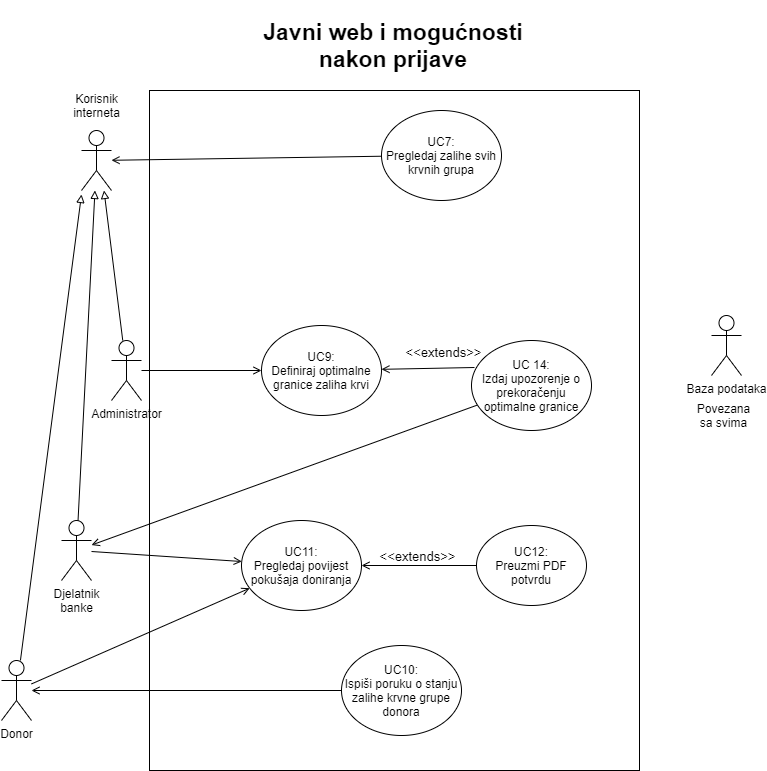
\includegraphics[scale=0.6]{slike/UC5.png} %veličina slike u odnosu na originalnu datoteku i pozicija slike
    			\centering
    			\caption{Dijagram obrazaca uporabe 5 - Javni web i mogućnosti nakon prijave}
    			\label{fig:promjene}
    	    	\end{figure}
    	    	
				\begin{figure}[H]
    			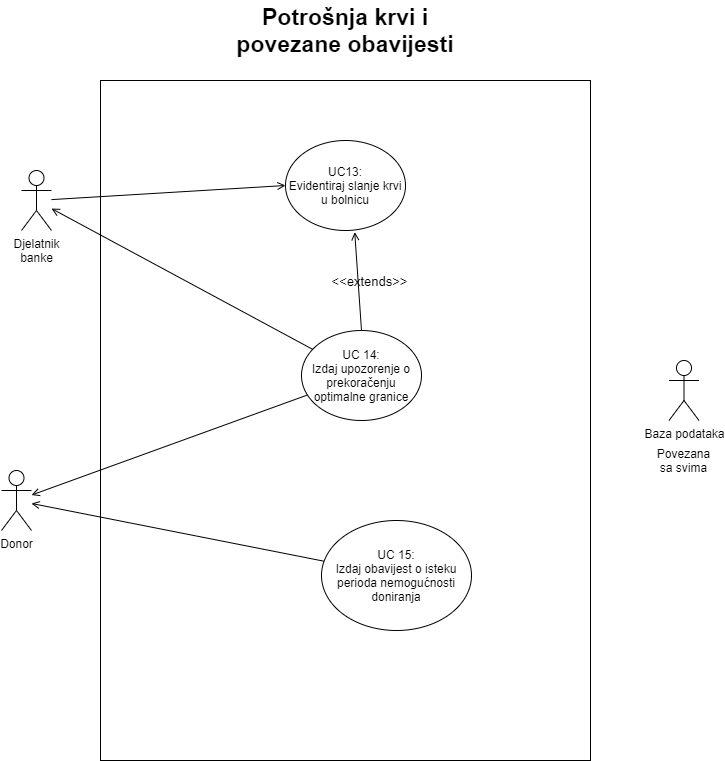
\includegraphics[scale=0.6]{slike/UC6.png} %veličina slike u odnosu na originalnu datoteku i pozicija slike
    			\centering
    			\caption{Dijagram obrazaca uporabe 6 - Potrošnja krvi i povezane obavijesti}
    			\label{fig:promjene}
    	    	\end{figure}
    	    	
				\eject		
				
			\subsection{Sekvencijski dijagrami}
				
				%\textbf{\textit{dio 1. revizije}}\\
				
				%\textit{Nacrtati sekvencijske dijagrame koji modeliraju najvažnije dijelove sustava (max. 4 dijagrama). Ukoliko postoji nedoumica oko odabira, razjasniti s asistentom. Uz svaki dijagram napisati detaljni opis dijagrama.}
				
				
				\begin{figure}[H]
    			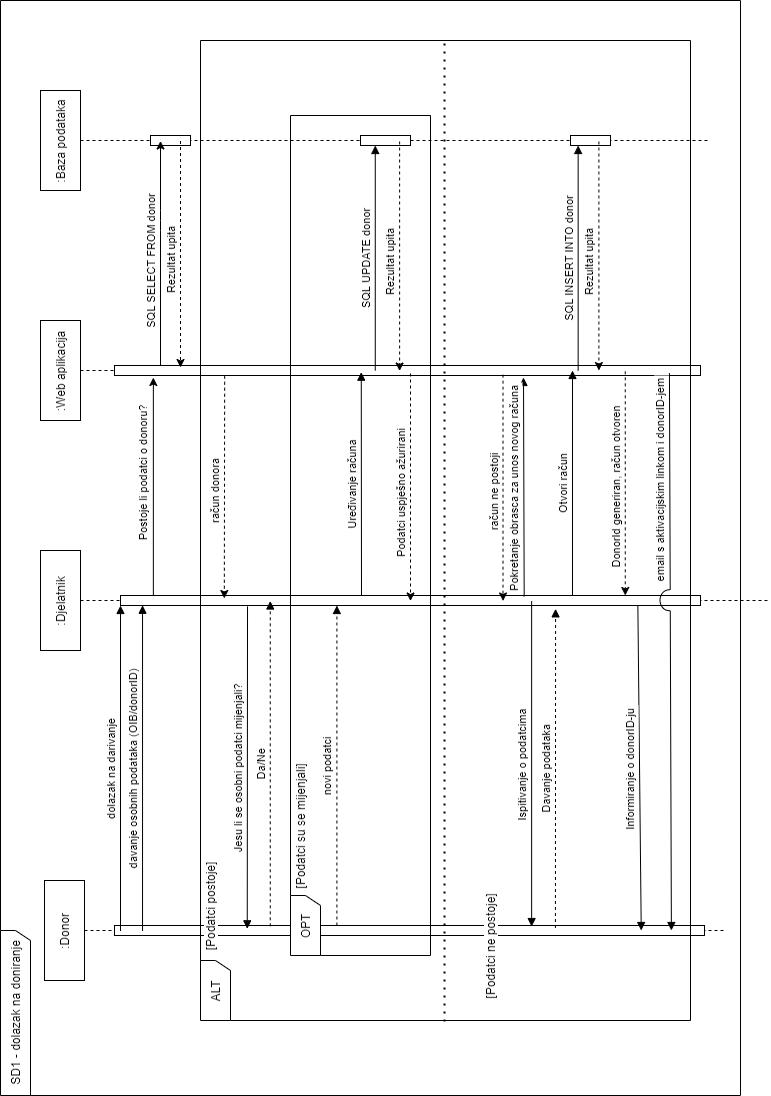
\includegraphics[scale=0.7]{slike/SD1_rot.png} %veličina slike u odnosu na originalnu datoteku i pozicija slike
    			\centering
    			\caption{Sekvencijski dijagram 1 - Potrošnja krvi i povezane obavijesti}
    			\label{fig:promjene}
    	    	\end{figure}
    	    	
    	    	\par {
    	    	    Sekvencijski dijagram 1: Donor dolazi na akciju darivanja krvi i djelatniku banke daje neki 
identifikacijski podatak (OIB ili donorID, ukoliko ga posjeduje).
Djelatnik banke provjerava postoji li u sustavu donor s tim podatkom (koji je
jedinstven za svaki račun). Web aplikacija djelatniku banke daje odgovor slanjem
upita u bazu podataka. Ukoliko podatci postoje, djelatnik banke u komunikaciji s 
donorom provjerava jesu li se podatci mijenjali i ažurira ih ako jesu.
U slučaju promjene, sustav ažurira podatke u bazi podataka.
Ukoliko nema postojećih podataka, sustav to dojavljuje djelatniku, koji kreće
u proces kreiranja novog računa. Djelatnik banke donora ispituje o osobnim podatcima,
unosi ih u sustav koji te podatke unosi u bazu podataka. Generira se donorID,
o kojemu djelatnik banke izvještava donora. Sustav također šalje e-mail s generiranim
podatcima o računu i poveznicom za aktivaciju računa.
    	    	}
    	    	
				\begin{figure}[H]
    			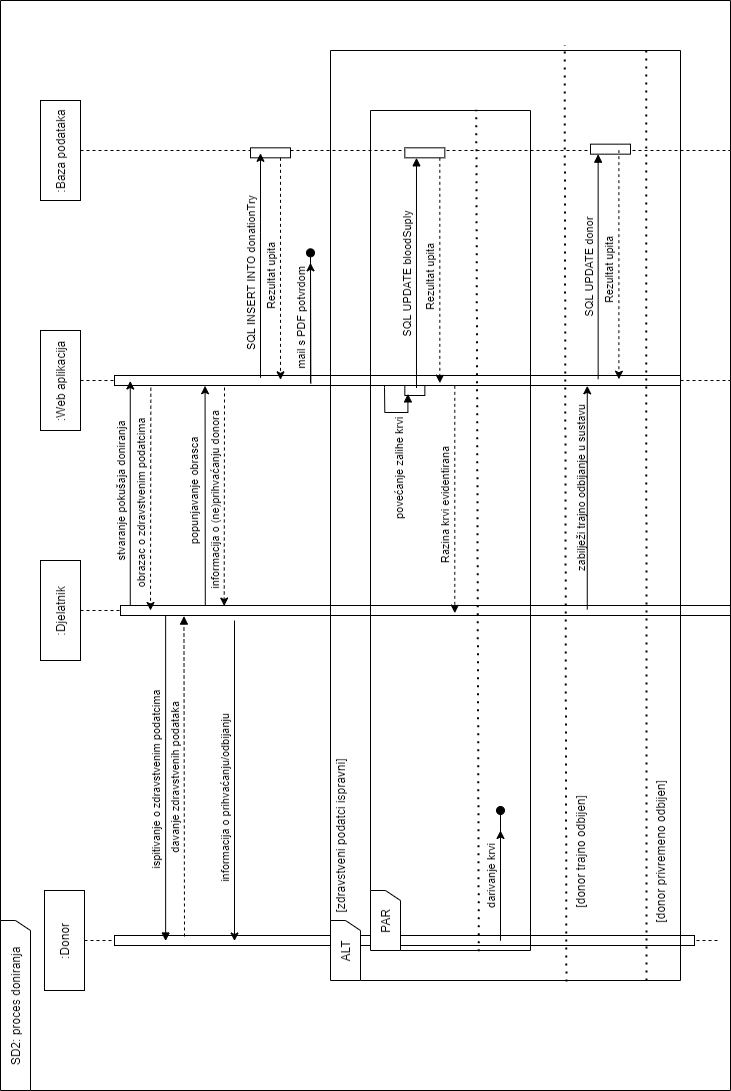
\includegraphics[scale=0.7]{slike/SD2_rot.png} %veličina slike u odnosu na originalnu datoteku i pozicija slike
    			\centering
    			\caption{Sekvencijski dijagram 2 - Potrošnja krvi i povezane obavijesti}
    			\label{fig:promjene}
    	    	\end{figure}
				
				\eject
				
				\par {
    	    	   Sekvencijski dijagram 2: Nakon provjere postojanja i ispravnosti podataka u sustavu, djelatnik banke za
donora stvara pokušaj doniranja. U obrazac koji se otvara u web aplikaciji
djelatnik banke evidentira zdravstvene podatke koje otkriva u komunikaciji s 
donorom (ili iz popunjenog obrasca koji mu dostavi donor).
Ukoliko neki od podataka implicira nemogućnost donora za darivanje krvi,
djelatnik banke donora informira o tome. Pokušaj doniranja sprema se u bazu podataka
te se donoru na mail šalje potvrda o pokušaju doniranja.
U slučaju da je donor nije odbijen (zdravstveni podatci su ispravni), u
sustavu se povećava zaliha krvi za jednu dozu ažuriranjem podataka u bazi, a
donor odlazi donirati krv.
U slučaju da je donor trajno odbijen, djelatnik banke dodatno u njegovom računu zabilježava
trajno odbijanje ažuriranjem donorovih podataka u bazi.
Ako je donor samo privremeno odbijen, ne poduzimaju se nikakvi dodatni koraci.
    	    	}
				
				
				
	
		\section{Ostali zahtjevi}
		
			%\textbf{\textit{dio 1. revizije}}\\
		 
			 %\textit{Nefunkcionalni zahtjevi i zahtjevi domene primjene dopunjuju funkcionalne zahtjeve. Oni opisuju \textbf{kako se sustav treba ponašati} i koja \textbf{ograničenja} treba poštivati (performanse, korisničko iskustvo, pouzdanost, standardi kvalitete, sigurnost...). Primjeri takvih zahtjeva u Vašem projektu mogu biti: podržani jezici korisničkog sučelja, vrijeme odziva, najveći mogući podržani broj korisnika, podržane web/mobilne platforme, razina zaštite (protokoli komunikacije, kriptiranje...)... Svaki takav zahtjev potrebno je navesti u jednoj ili dvije rečenice.}
			 
			 \begin{itemize}
			     \item Sustav treba omogućiti rad više korisnika
			     \item U sustavu treba postojati tri vrste korisnika - donor, djelatnik banke i administrator
			     \item Aplikacija mora biti izvedena kao web-aplikacija
			     \item Aplikacija mora biti prilagodljiva različitim veličinama ekrana te mobilnim uređajima
			     \item Autentikacija korisnika radi se korisničkim imenom (donorID) i lozinkom
			     \item Lozinke u sustavu moraju biti enkriptirane radi zaštite u slučaju neovlaštenog pristupa
			     \item Lozinke korisnika moraju biti dovoljno sigurne radi sprječavanja neovlaštenog pristupa računu (trebaju imati bar 2 od 4 zahtjeva - mala slova, velika slova, brojevi, specijalni znakovi) 
			     \item Računi su pri stvaranju neaktivirani, a aktiviraju se aktivacijskim linkom dostavljenim u e-mailu koji se šalje pri kreiranju računa na e-adresu navedenu pri kreiranju računa
			     \item Sustav korisnicima ne smije otežavati rad, stoga mora biti napravljen intuitivno i kao jednostavan za korištenje
			     \item Sustav mora biti otporan na pogreške, ne smije se srušiti, nego treba dojaviti pogrešku i omogućiti izmjenu neispravno unesenih podataka
			 \end{itemize}
			 
			 
			 
	